HTBAC serves as a software tool to enable ensemble-based free energy protocols
to run adaptively and at scale. \mtnote{protocols?}\jdnote{addressed}.
% HTBAC is based on a co-design which integrates users i.e. domain experts and
% developers to elicit requirements.


% \mtnote{I am not sure I understand what this
% means. Domain experts and developers both elicit requirements? What about the
% rest of the development process? The sentence's grammar also needs
% attention}.

% The co-design process is iterative. For example, certain features become
% available during the software lifetime which in turn can be used by domain
% experts to build new algorithms that require such features.

% ---------------------------------------------------------------------------
\subsection{Requirements}

HTBAC has three primary requirements: (1) enable the scalable execution of
concurrent free energy protocols; (2) abstract the complexity of building
protocols
% \mtnote{``from'' instead of ``,''? See also comment in the
% following paragraph} 
from execution and resource management; and, (3) provide
adaptive features by modifying the task-graph, to enable protocols to run more 
efficiently during runtime.  

% (i.e., modifying the task-graph at runtime, based on
% previous tasks), to enable efficient protocols and effective resource sharing
% across and within protocols. 
% without explicit resource management requirements.

Based on the requirements of computational drug campaigns \mtnote{which
one?}\jdnote{keeping it general to campaigns} 
which requires the ability to run multiple concurrent protocols in order to 
scale the number of drug candidates or protein ligand systems, this poses 
challenges in the coordination of heterogeneous protocols that differ in 
computational requirements as well as setup of execution environments and data
management, while preserving efficient resource utilization. 
\jdnote{reworded this paragraph}
% and minimal overhead
% workload management system and the runtime system 
% (RTS) that support HTBAC.

% \mtnote{I am not sure I understand this sentence: grammar
% (``Based\ldots,this''?; and from the previous paragraph, we say that HTBAC
% abstracts the complexities of execution and resource management but here we
% focus on WMS and RTS? Are WMS and RTS components of HTBAC?} 

% The RTS has to
% provide sustainable submission and tracking of heterogeneous protocols
% i.e.\mtnote{note: ``i.e.'' cannot be place in the middle of a sentence
% without supporting punctuation} 
% protocols that differ in computational
% requirements, as well as setup of execution environments and data management
% while preserving efficient resource utilization and minimal
% overhead.\mtnote{Why this is relevant for HTBAC?}

Usability plays an important role in the development of HTBAC, in order to
provide a flexible interface which enables users to easily scale the number
of drug candidates and quickly prototype existing and novel free energy
protocols.

Based on intermediate results during runtime, the control logic of the
algorithm may decide to invest additional computational resources in more
interesting simulations that can yield higher accuracy, while reducing
resources for simulations that have already met their accuracy threshold.
HTBAC thereby requires an adaptive runtime system \mtnote{system}
\jdnote{addressed} that enables adaptive algorithms to maximize computational
efficiency.\mtnote{Seeing that we are speaking about requirements, does it
make sense here to mention a RTS? RTS are an implementation detail: for
example, we could design HTBAC as an end-to-end solution for a specific
machine and still match the set of requirements we have reported in this
subsection. Note also that we introduce RTS above but use ``runtime system''
again here.}\jdnote{I've removed all mention of workload management system 
and RTS and kept generality in runtime system}

% ---------------------------------------------------------------------------
\subsection{Design}

We model an application in HTBAC\mtnote{what is an ``application of HTBAC''?
`In' (instead of `of') HTBAC?}\jdnote{addressed} using the following user-facing 
constructs:

\begin{itemize}
  \item \textbf{Protocol:} A generic abstraction of a free energy protocol
  such as ESMACS or TIES.
  \item \textbf{Simulation:} Simulation parameters that supply additional
  information for each protocol instance.
  \item \textbf{Runner:} Cyber-infrastructure resource abstraction for the
  application.\mtnote{``resource abstraction of the application''? Resources
  for the application?}\jdnote{addressed}
\end{itemize}

The \textbf{Protocol} component \mtnote{we used `construct' before, as a synonym
of abstraction}\jdnote{I've removed any reference to object-orientation and kept
everything to components} enables multiple instantiations of protocol types. 
The \textbf{Simulation} component \mtnote{we used `construct' 
before, as a synonym of abstraction} specifies simulation parameters that shape 
each protocol. The \textbf{Runner} component provides the functionality to 
specify the resource and temporal requirements of the application.

An HTBAC application contains one or more protocol instance(s) which can execute 
independently and concurrently. 


% The replica subcomponent defines the number of ensemble members for a
% given protocol instance, while the system subcomponent defines the input
% configuration files necessary to execute the protocol instance. 

\jdnote{move this next section to description of implementation}

%  -----------------------------------------------------------------------------

% Each protocol follows the same initial sequence of simulation
% steps including minimization, equilibration and production simulation.\mtnote{see
% the previous comment about using `i.e.'}\jdnote{addressed}

% Protocols differ only 
% by their individual analysis step which typically follows production simulation 
% and by the computational requirements, 


% see figure X for a visual representation of
% the ESMACS and TIES workflows \mtnote{grammar. I am not able to follow the
% sentence}.


% Moreover the
% \textbf{Simulation} class provides the granularity to specify individual
% parameters per replica, including the number of cores per replica, MD
% execution kernel and the length of each simulation step.\mtnote{This might be
% seen more as a description of the implementation of HTBAC instead of its
% design}\jdnote{moved this to TIES description of implementation}

% Note that some protocols require additional information. For example, the
% TIES protocol contains additional sampling parameters or $\lambda$ windows.
% Moreover, the \textbf{Simulation} class exposes a method which enables the
% user to codify new algorithms, or modify an existing protocol such as
% specifying additional equilibration or analysis steps.\jdnote{move to 
% implementation}

% Once the protocols and simulation parameters are defined, they are passed to
% the \textbf{Runner} class where the user defines the resource requirements
% including cyber-infrastructure and duration of the application as well as
% additional flags for adaptive execution which are passed down by the
% \textbf{Runner} to the workload management and runtime systems.\mtnote{This
% seems to be mixing implementation, execution flow and architecture?}
%  -----------------------------------------------------------------------------


\mtnote{General note. It may be useful to recall the difference between
software architecture and software design. Software architecture is about the
structure of the software system, with a particular focus on modularity and
how it is rendered by components and interfaces (e.g., communication and
coordination protocols). Software design is about defining the
functionalities of each module, \textbf{showing} (i.e., arguing for) how
these functionalities address the requirements. In this context, the notion
of `class' and `method' are often regarded as implementation details, even if
object-oriented design is indeed one of the many ways to approach software
design. More in general, both architecture and design can be expressed with a
varying degree of formality and many different patterns and languages have
been and are still being developed. In this paper, we just use plain English,
informal diagrams, and a very high level overview. This approach should not
be confused with lack of precision or of scientific rigor: the goal of this
paper is to show how HTBAC architecture and design support better science in
a very specific domain, not to argue for their rigorous nature.}
\jdnote{I've modified the design to be more consistent in showing functionality
of components}

% For TIES, where each protocol  corresponds to a single physical system. The
% TIES protocol object enables the user to select a physical system, number
% of replicas, core allocation per replica, and $\lambda$ windows to sample.
% Figure~\ref{fig:pst} provides the visual implementation of the TIES
% protocols into the PST model.

% ---------------------------------------------------------------------------
\subsection{Implementation}

% The \textbf{Protocol} construct is the main abstraction of HTBAC. 

Each protocol represents a protein ligand system \mtnote{see the
previous comment about using `i.e.'}\jdnote{removed i.e.}. A protocol 
defines a % simulation 
pipeline composed of an ordered sequence of simulation steps. In
ensemble-based, free energy protocols such as ESMACS or TIES, these
pipelines are replicated, where replicas differ by their parameter
configurations. For example, in ESMACS and TIES, replicas only differ by initial
velocities, which are assigned randomly by the MD engine at the start of
execution. By nature of ensemble applications, each replica within a protocol
can execute its pipeline independently. We model a simulation step in a 
replica as a computational \textbf{task}, which has a defined input, output, 
termination criteria and dedicated resources~\cite{power-of-many17}. Aggregates 
of tasks with dependencies describe workflows

A computational
\textbf{task} represents an independent simulation. Aggregates of tasks
create \textbf{workflows} 

HTBAC is implemented in Python, and uses RADICAL-Cybertools (RCT) to provide
ensemble-execution capabilities and a runtime system to execute protocols.
The RCT are middleware building blocks~\cite{review_bb_2016} engineered to
support the execution of extensible and scalable workflows across diverse
computing platforms~\cite{turilli2017comprehensive}. HTBAC rests on two
primary RCT components, Ensemble Toolkit (EnTK) and RADICAL-Pilot (RP).

\jdnote{maybe mention something about domain specificity}

\begin{figure}
  \centering
  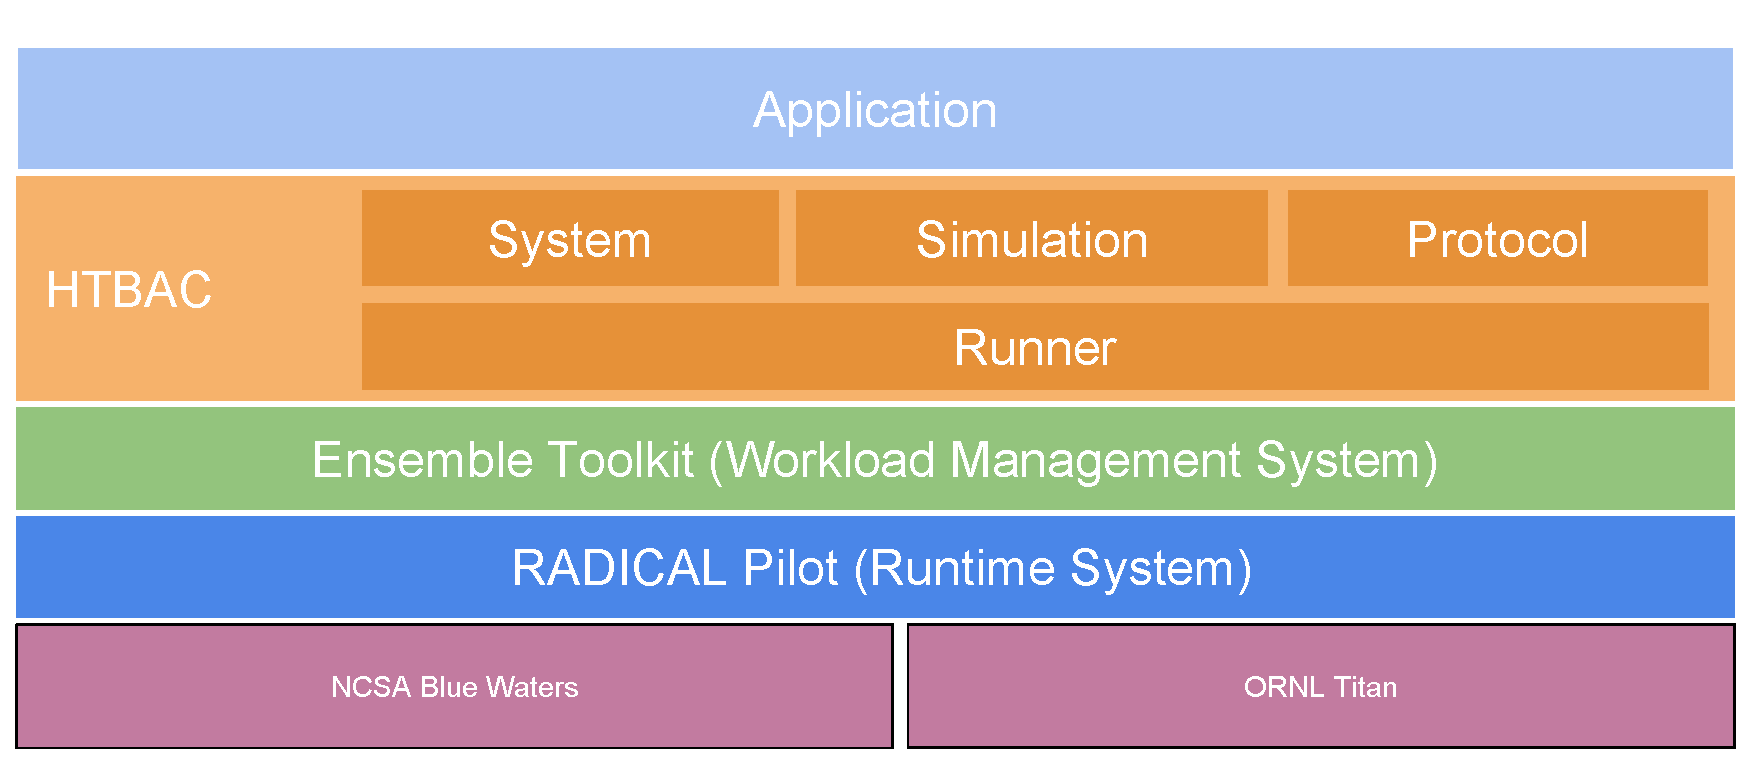
\includegraphics[width=\columnwidth]{figures/building_blocks.pdf}
  \caption{Layered architecture of HTBAC, EnTK, and RP. The HTBAC API
  exposes the Protocol component. Current protocols supporting the use cases
  include ESMACS and TIES. EnTK serves as the workload execution system.
  RADICAL-Pilot serves as the runtime system.}
\label{fig:blockdiagram}
\end{figure}

Figure~\ref{fig:blockdiagram} shows a visual block diagram representation
\mtnote{`visual block diagram representation' seems unclear to me. Should we
just have an architecture diagram here?} of HTBAC and the underlying building
blocks.

(include the mapping of protocols to PST model maybe using a better
diagram)\mtnote{is this a comment? Please clearly identify comments in the
text.}

% ---------------------------------------------------------------------------
\subsection{Workload Management and Runtime System}

EnTK simplifies the process of creating ensemble-based applications with
complex coordination and communication requirements. The EnTK API exposes the
PST model which consists of three components\mtnote{I am not sure these are
components. There is the risk to consider them architectural elements when
they are not}: \textbf{Pipeline}, \textbf{Stage}, and \textbf{Task}. HTBAC
promotes binding affinity \textbf{Protocols} as the user-facing construct,
and uses the programming model defined by the Pipeline, Stage and Tasks model
to express a specific protocol. \mtnote{The second part of this paragraph is
inconsistent with the first: for example, see the use of PST and then
`Pipeline, Stage and Task', or the use of protocols with capitalization
(proper names are not plural) without differentiating them (it?) from those
defined in EnTK via PST}

% Each HTBAC application aggregates one or more protocols. A workflow is
% comprised of $N_P$ instances of the P$^{th}$ protocol.

% each stage is a computational \textbf{task}, and the ordered aggregation of
% these stages alongside their dependencies as a
% \textbf{pipeline}~\cite{power-of-many17}.

% Sets of tasks with dependencies that determine the order of their execution
% are usually referred to as “workflows”.

% In section \ref{sec:science-drivers}, we described two examples of
% ensemble-based protocols for computing binding affinities.

Once the workflow is described \mtnote{the previous paragraph does not
mention workflow(s) so this surprises and confuses the reader. Note that this
is a byproduct of commenting out part of the text where a connection between
protocol and workflow was explicitly established}, protocols are translated
into EnTK pipelines, and are submitted to EnTK's \textbf{Application Manager}
which sets up multiple processes, threads and a RabbitMQ message queue for
communication. EnTK identifies tasks which have satisfied dependencies and
can be executed concurrently. EnTK's \textbf{Execution Manager} uses the
underlying runtime system (RADICAL-Pilot) to execute the tasks on specific
target resources.

EnTK converts the set of pipelines into a set of tasks---called compute unit
descriptions---and submits them to RP \mtnote{Is RP defined?}. In EnTK, a
Pipeline is created for each unique combination of the following parameters:
system, replica, and thermodynamic state i.e. $\lambda$ window in the case of
TIES~\ref{fig:ties_workflow} \mtnote{This paragraph overlaps in scope with
the last part of the previous paragraph. This results in repetition and
confusion for the reader. Also, note that punctuation is missing, including
the one closing the sentence.}

In addition, HTBAC passes the computational requirements \mtnote{of what?} to
EnTK which creates a resource request including walltime, cores, queue, and
user credentials. EnTK converts this resource request into a pilot that RP
submits to a HPC machine. Once the pilot becomes active, it pulls compute
unit descriptions in bulk from a database, executing them on the pilot
resources.\mtnote{This paragraph reads as a leftover, partially overlapping
with what already explained. It requires better integration with the previous
two paragraphs.}

\begin{figure}
  \centering
  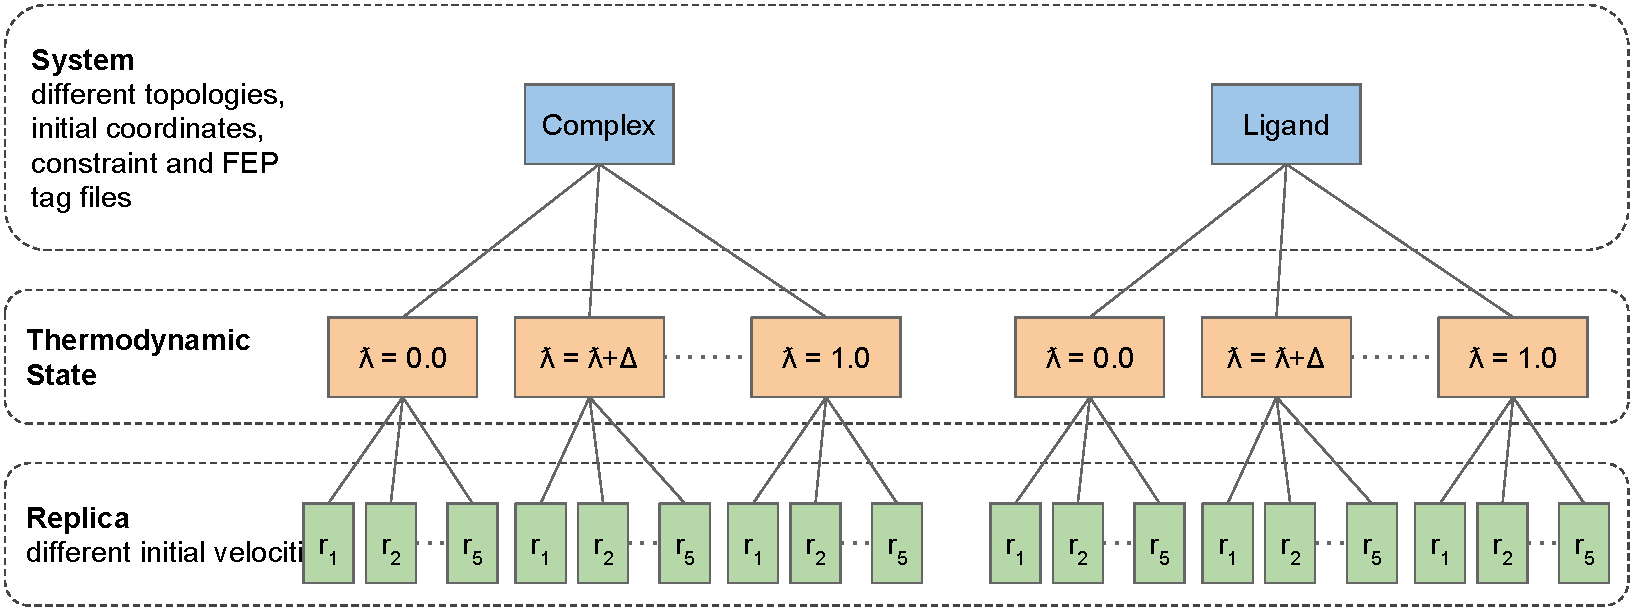
\includegraphics[width=\columnwidth]{figures/ties_workflow.pdf}
  \caption{TIES workflow consisting a physical system, thermodynamic states
  and replicas. Each replica is assigned a thermodynamic state. The workflow
  is translated into an EnTK PST workflow. Construction Number of EnTK
  Pipelines = 2 * (($\lambda$(max)/$\delta$) + 1) * 5 where $\lambda$(max) =
  1 }
\label{fig:ties_workflow}
\end{figure}

  
\begin{figure}
  \centering
  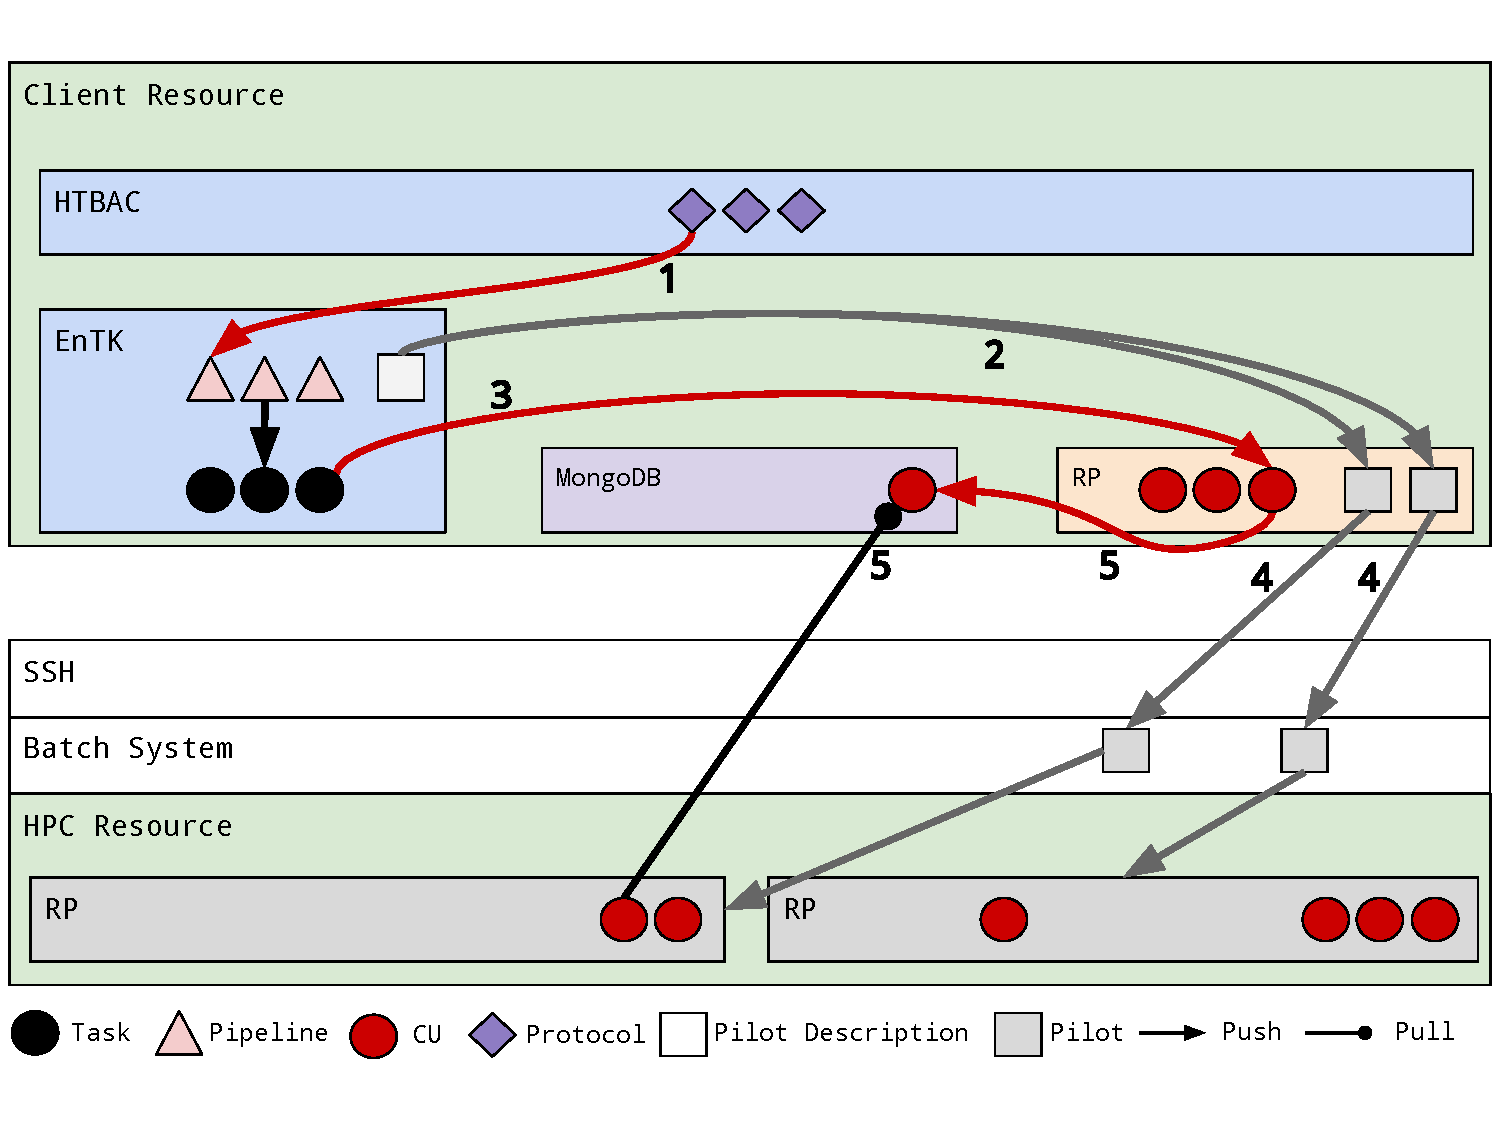
\includegraphics[width=\columnwidth]{figures/ht-bac-rp_integration.pdf}
  \caption{Ensemble Toolkit (EnTK) and RADICAL-Pilot (RP) architecture and
  execution model.\mtnote{Unreferenced figure.}}
\label{fig:integration}
\end{figure}

% Consistent with EnTK's programming model, HTBAC also uses the PST model to
% express {\bf Protocols}.

% Each protocol contains multiple stages with simulations and analysis tasks
% interspersed, in the most general case.

% programming model (that are consistent with the EnTK) to enable the user 

% HTBAC rests upon established middleware solutions~\cite{review_bb_2016},
% validated runtime abstractions~\cite{turilli2017comprehensive} for scalable
% execution, and customizes them for the computation of binding free
% energies.

% HTBAC derives many of the advantages of a lightweight, flexible domain
% specific workflow layer from its use of RADICAL-Cybertools (RCT) which are
% functionally well-defined and delineated middleware building blocks.
% RCT~\cite{review_bb_2016} are engineered to support extensible and scalable
% workflows across diverse computing platforms. The two primary RCT
% components that HTBAC depends upon are the Ensemble Toolkit (EnTK) and
% RADICAL-Pilot (RP).

% (so far, a workflow entails a maximum value of $P = 2$ and $N_P$=16, but in
% future work P will be greater $>$ 2).

% protocol, a user can scale protocol instances to study as many physical
% systems as desired.

% The specification of protocols and their parameters are passed by the user
% to the \textbf{Runner Handle} which translates the request to EnTK.

% In Section \ref{sec:related-work} we highlighted how an ensemble simulation
% approach can both aid sampling and improve uncertainty quantification for
% free energy calculations. Despite these crucial advantages, it remains
% non-trivial for field researchers to write biosimulation applications that
% involve individual protocols supporting multiple replicas, and by extension
% multiple protocols. With HTBAC, this burden is minimized by specifying the
% number of concurrent instances of the \textbf{Protocol} object. Moreover,
% the ability to generate multiple protocol instances enables the user to
% investigate a range of physical systems (i.e., drug candidates)
% concurrently.

% HTBAC allows the simple expression and concurrent execution of multiple
% distinct protocols, thereby enabling concurrent screening of drug
% candidates. HTBAC not only simplifies the expression of complex binding
% affinity protocols, but also provides hitherto unavailable capabilities,
% viz., the adaptive execution of these protocols, without any additional
% programming burden.

Explain adaptive API and how it is passed to EnTK\mtnote{Please clearly
identify comments in the text.}

% In turn, our adaptive execution implementation at the WMS focuses on
% supporting generality of adaptive workflows at the inter and intra-protocol
% level.

% \begin{figure}
%   \centering
%    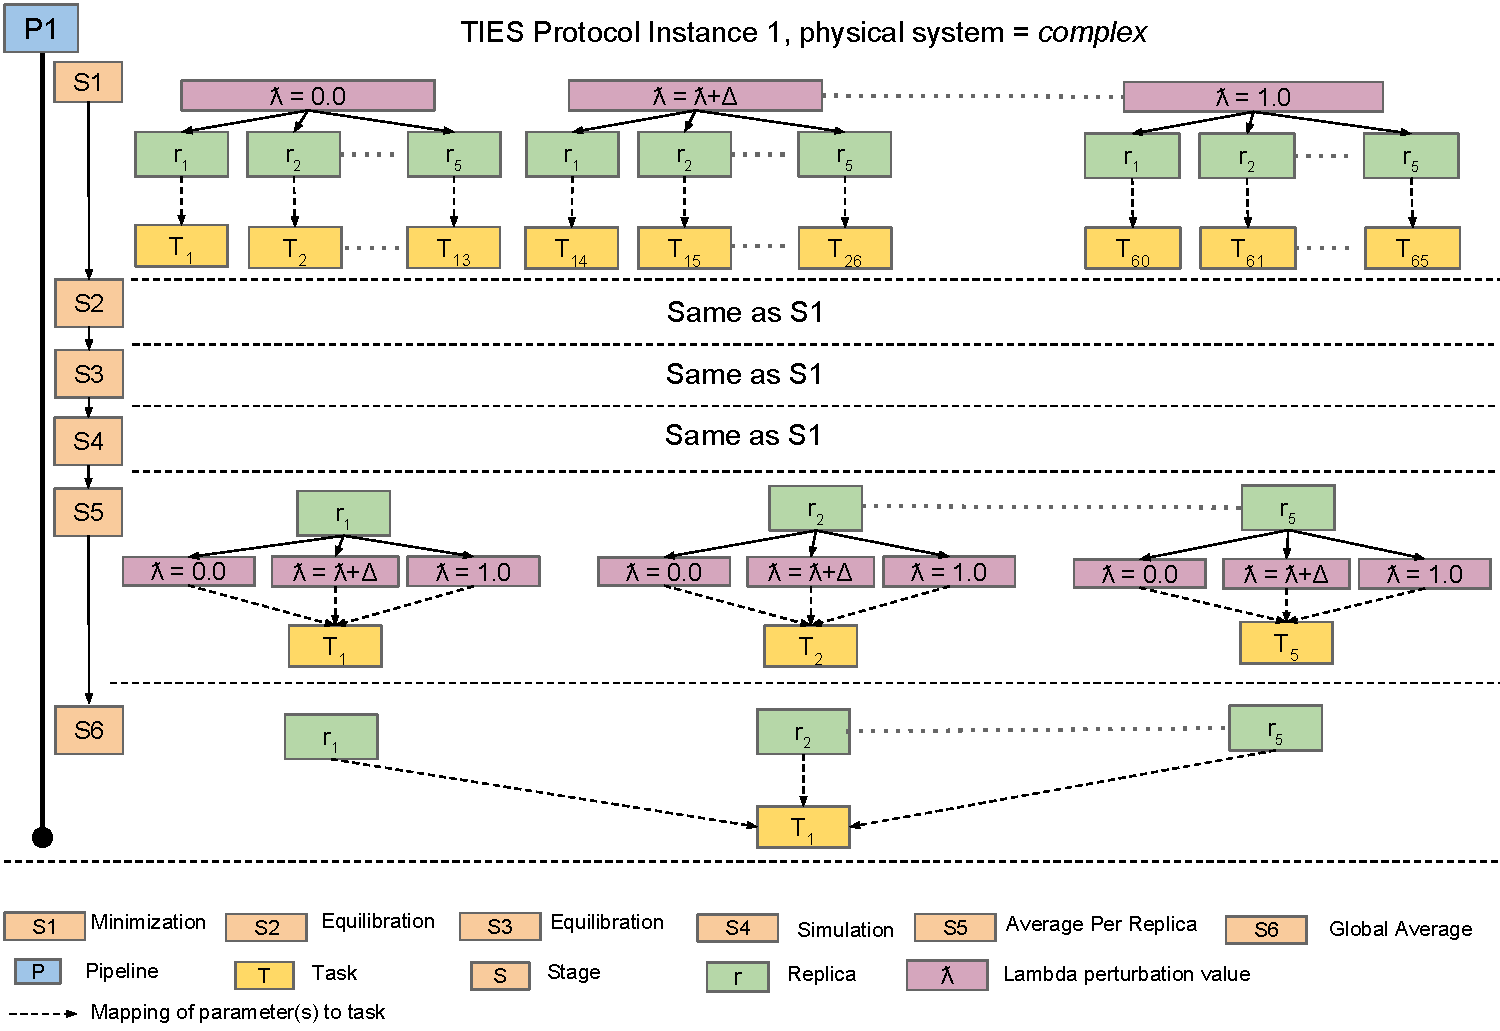
\includegraphics[width=\columnwidth]{figures/_TIES_EnTK_implementation.p
%    df}
%   \caption{TIES protocol expressed using the EnTK PST model. Each protocol
%   instance maps to a single Pipeline, comprised of Stage(s) which maintain
%   temporal order. Each Stage executes $n$ tasks, where $n$ represents the
%   number of unique lambda-replica combinations.}
% \label{fig:pst}
% \end{figure}


% \subsection{Scalability}

% Each protocol instance studies a single physical system i.e. drug
% candidate. By extension, the user is able to scale the number of concurrent
% protocol instances and therefore explore multiple concurrent drug
% candidates.

% ---------------------------------------------------------------------------
\subsection{Adaptivity}

In section~\ref{sec:science-drivers}, we described a particular type of
adaptivity within TIES that would enable the simulation \mtnote{which one? Or
should this be `a simulation' or `simulations'?} to reach convergence
earlier. Figure~\ref{fig:adaptive_ties} illustrates the adaptive workflow of
TIES (change $\lambda$ step size as $\delta$ \mtnote{is this a comment?
Please clearly identify comments in the text.}). Adaptive execution requires
changes to the task graph during runtime, a capability supported by the RCT
runtime layers~\cite{power-of-many17}.

The TIES adaptive workflow decides, postmortem \mtnote{no dash}, about the
placement of new $\lambda$ windows for the next set of simulations. In turn,
the workflow makes runtime decisions about the number of tasks in the task
graph. This type of adaptivity in the workflow requires as \mtnote{as what?
Requires capabilities to count tasks and changing the attribute of tasks
depending on \ldots?} task-count and task-attribute
adaptivity~\cite{adaptivebiomolecular}.

HTBAC monitors the output of the completed tasks during runtime, and
redefines the existing workflow by adding more $\lambda$ windows \mtnote{as
required? The sentence appears to be incomplete}. A boolean results generated
at the end of a pipeline defines a criteria of whether or not
\mtnote{when using `whether' the `or not' is implied} to spawn additional
tasks.

% Spawning of new task contribute to task count adaptivity and task attribute
% adaptivity. Using EnTK, HTBAC creates the necessary set of new tasks.

The \textbf{Application Manager} in EnTK signals RP to bypass termination of
the pilot and instead keep the session alive, as long as additional tasks are
submitted. As the number of tasks grows during runtime, the ratio of
core-to-task fluctuates. HTBAC exposes the core allocation per task, and
allows users to specify before runtime the resource requirements of
additional tasks.\mtnote{I tried to fix a bit the paragraph but it still
difficult to read and understand.}

\begin{figure}
  \centering
  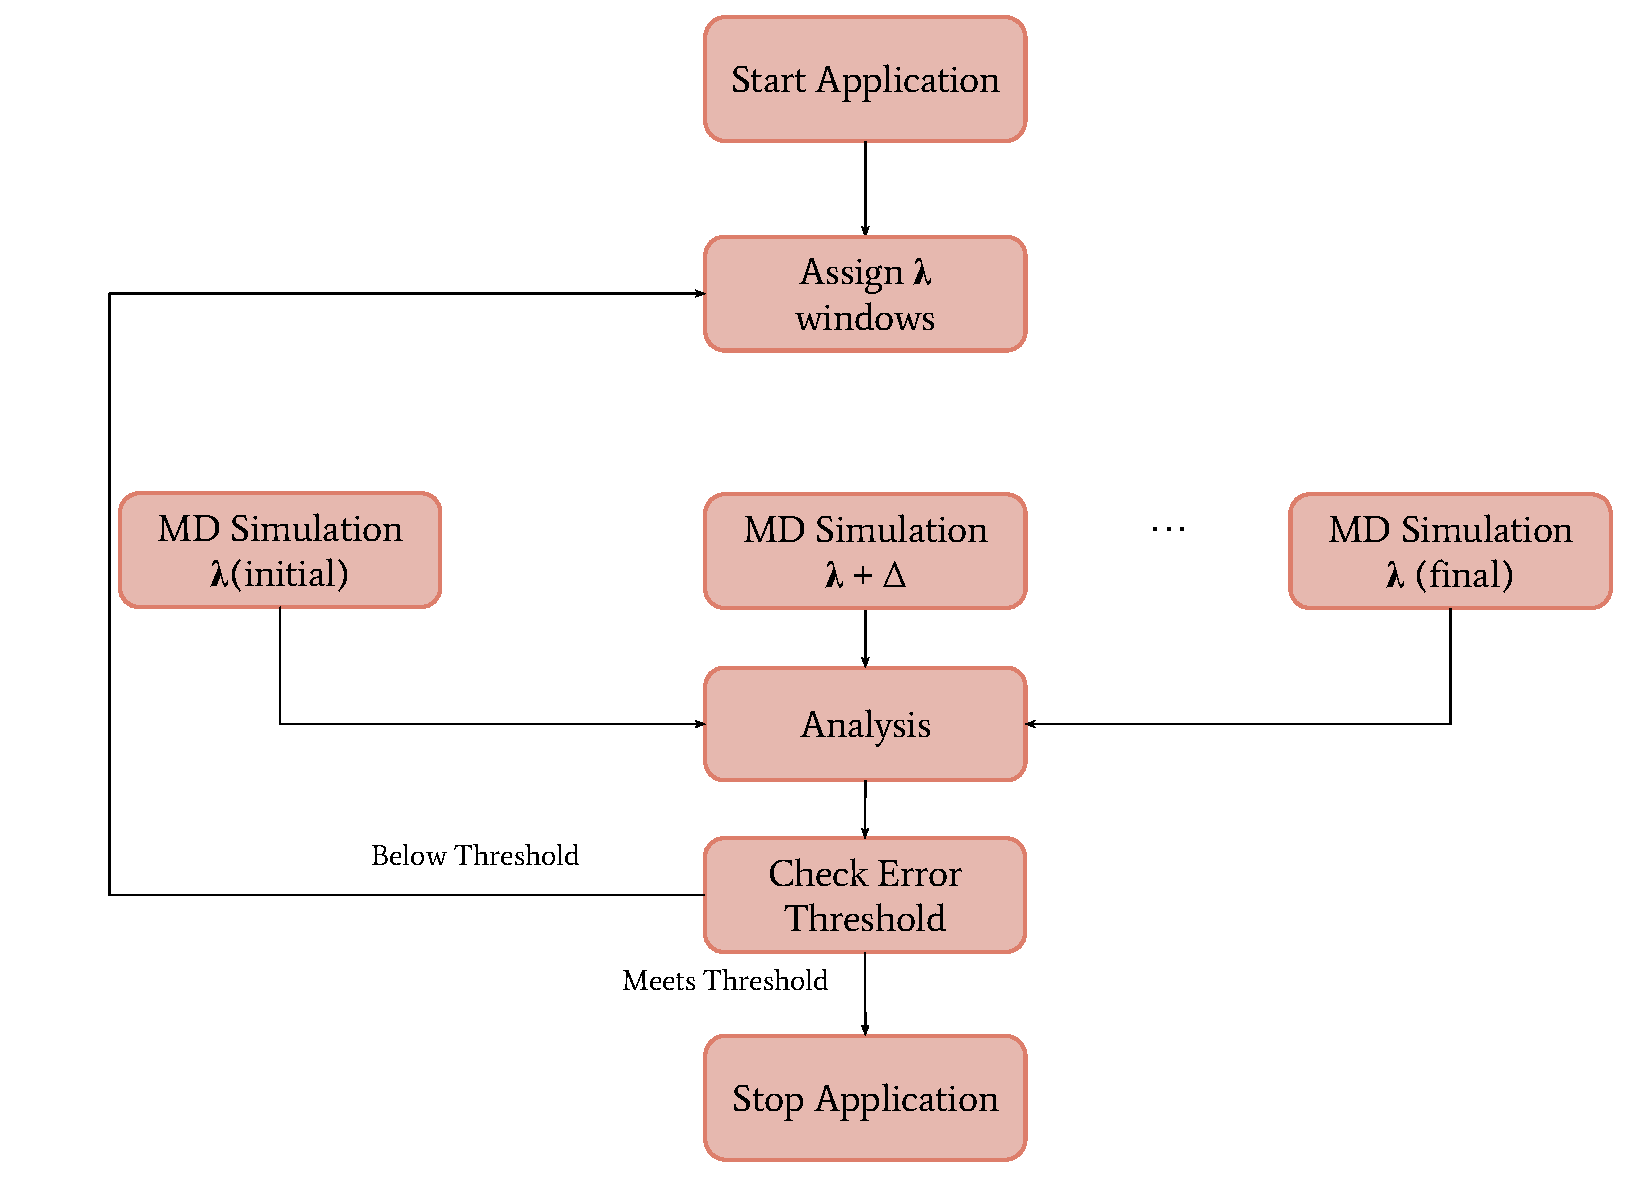
\includegraphics[width=\columnwidth]{figures/adaptive_TIES_workflow_diagram.pdf}
  \caption{Adaptive workflow of TIES consisting of multiple concurrent and
  independent simulations. The analysis step operates on a snapshot of the
  current simulations for each $\lambda$ window, and decides if the critical
  threshold is reached, else the current simulations continue executing and
  new simulations are spawned based on additional $\lambda$ values.}
\label{fig:adaptive_ties}
\end{figure}

%\jhanote{Is this specific to the TIES protocol or to the protocol class.
%Needs clarification.} The same approach has been expanded to facilitate the
%creation of sub-ensembles where the simulation configuration is altered
%programatically. An example of this is the implementation ofthe TIES
%protocol, where the user controls the $\lambda$ parameter values used in
%simulatios to control which hybrid system states are sampled.

%A parameter, $\lambda \in [0, 1]$ is set for values between extremes and a
%simulation has to be run for every $\lambda$ value. The values form a
%function of energy and are integrated to obtain the desired results, the
%\emph{relative} binding free energy.

% ---------------------------------------------------------------------------
%\subsubsection{System}

%Systems This allows for multiple systems to be tested in the same
%\emph{single} run. A common scenario is the calculations of the binding
%affinity of a set of ligands with the same protein. System itself is just a
%collection of file paths pointing to descriptions of the system, like the
%system structure, topology etc. This class also provides the core/node
%requirments per single run, and reads some of the system descriptions from
%files to fill in the configuration settings.

%The Pipeline-Stage-Task (PST) framework developed by the Radical team
%(cite), and the Ensemble Toolkit (EnTK) built on top of it, offers a
%flexible way to express the molecular dynamics simulation workflows present
%in academia (cite) in terms of the radical pilot execution environment. Here
%we present a proposed mapping between the two (the PST and the MD layers)
%that is both simulation engine and protocol agnostic and allows for the
%compact expression of ensembles frequently used in binding affinity
%calculations.

%\subsection{Overview}

%The framework, called High Throughput Binding Affinity Calculator (HT-BAC),
%a python library, is made up of the following components: Workflow, Step,
%Ensembles and Simulation. These four object are all that is neccessary to
%describe the complex binding affinity caluculations in a generic way.

%\subsection{Workflow}

%The highest level abstraction is the Workflow. It is a container for the
%sequential units that are the simulation steps themselfs, and also contains
%meta-information about the job, like the resource description that the job
%will be running on, the total number of cores (nodes) required to fullfil
%the needs of the simulations and profiling mechanims to measure execution
%time.

% ---------------------------------------------------------------------------
%\jhanote{I don't these "description" should be subsections. Consider
%"\paragraph{}"}

%\subsection{Step}

%\jhanote{what is a step? It is unclear to the reader. Is "step"  construct
%within HTBAC or is this just a description of the pipeline?}

%The workflow containts an ordered list of \emph{steps}. Steps give
%\jhanote{order?} orderd to the basic building blocks of binding affinity
%calculations. Usually they are (i) minimization (some form of local
%optimization of atom coordinates), (ii) heating, (iii) equilibration and
%(iv) production run.

%Additionally there is one or more steps of analysis at the end. The key
%point, is that these steps \emph{have} to be run consecutively, as they are
%dependent on the previous one. This is ensured by the \texttt{Stage} objects
%of EnTK\@. Each step has list of \texttt{Ensemble}s and a
%\texttt{Simulation} object.

% ---------------------------------------------------------------------------

%$\subsection{Adaptability}

%Once we tackle the barrier between the local workflow creation and the
%remote execution, new features become availble, and readily usable by
%scientists. Intraprotocol adaptability is one such new feature.

% ---------------------------------------------------------------------------

% \subsubsection{Intraprotocol adaptability}

%while conceptually simple, tradiational execution patters used in academia
%makes this very hard. In HTBAC variables like replica size, specific lambda
%windows or simulatable system are settable on demand, the execution of which
%is automatically handeled by the library. To illustrate: a common scenario
%is the non adequate convergence of the statistical results after running a
%given number of replicas. In HTBAC the replica number can be changed, rerun
%and the results reevaluated. Additionally, logic can be written, to
%dynamically add more replicas until a given convergence tolerance has been
%reached.
